\documentclass[../main.tex]{subfiles}

\begin{document}
\section{Prior work}
\subsection{Camera array implementation}
The Raspberry Pi camera array, when initially implemented by Rafe Denham, achieved poor light field rendering quality \cite{denhamRaspberry} (see figure~\ref{fig:sum-squeeze-calibrated}). The calibration method used was one proposed by Vaish et al., and involves a \emph{plane + parallax} framework \cite{vaish2004using}. In Denham's evaluation, a definitive reason for the poor rendering quality is not provided, but it is suggested that it may have been due to an incorrect implementation of Vaish's algorithm.

\begin{figure}[H]
    \centering
    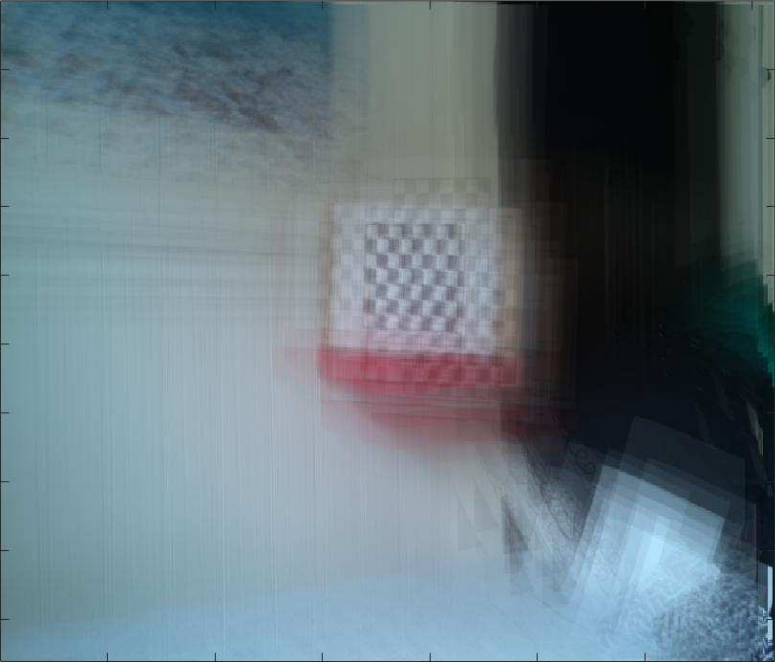
\includegraphics[width=0.85\linewidth]{images/sum-squeeze-rendering-calibrated}
    \caption{Light field calibrated using Vaish's plane + parallax procedure exhibiting poor focus. Adapted from \protect\bibentry{denhamRaspberry}}
    \label{fig:sum-squeeze-calibrated}
\end{figure}

After some testing of the original, we discovered that although the cameras appeared to be planar with a uniform viewing direction, in reality they exhibited significant arbitrary rotation, which Vaish's method does not account for. The lack of conformity in poses may have been at least partially related to the original medium-density fibreboard front-plate, which has since been replaced (see section~\ref{sec:front-plate-replacement}). However, even after replacing the front-plate, the cameras continue to retain significant arbitrary rotation (see figure~\ref{fig:rotation-evidence}).

\begin{figure}[H]
    \centering
    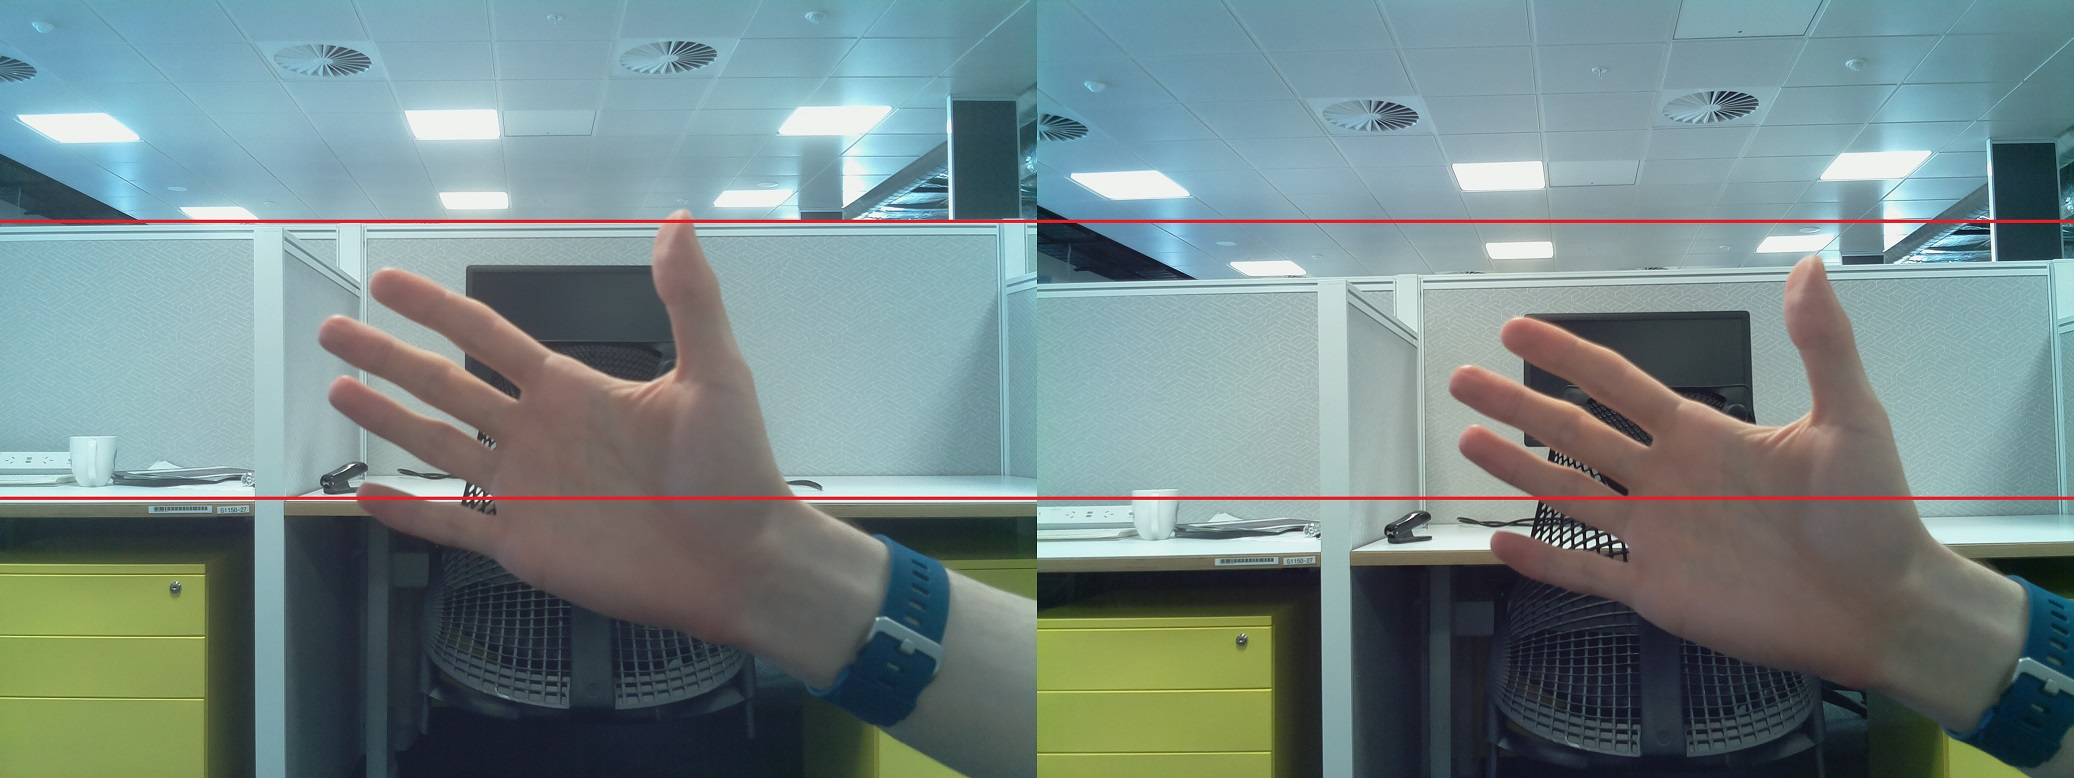
\includegraphics[width=\linewidth]{images/rotation-evidence}
    \caption{Images taken from two horizontally adjacent cameras in our camera array. The red lines illustrate the variance in camera orientation. This variance must be accounted for if calibrated light fields are to be generated.}
    \label{fig:rotation-evidence}
\end{figure}

\subsection{Calibration literature}
\subsubsection{Identifying the research gap}
Calibration procedures that facilitate light field acquisition can be categorised as either metric or non-metric. Metric calibration procedures recover precise camera positions and orientations. These methods are conceptually complex and take time to implement. Non-metric procedures, while simple, only recover camera positions to some unknown scale. However, it turns out that this is acceptable for most light field applications including 3D reconstruction, synthetic aperture imaging, light field rendering and space-time view interpolation. 

Vaish's \emph{plane + parallax} calibration procedure is the only non-metric light field camera calibration procedure that we are aware of. The procedure is one of the simplest procedures for light field acquisition, and it is currently used by Stanford University for their multi-camera array. The procedure requires each camera to be arranged on a plane. Images can then be projected onto a reference plane parallel to the camera plane, by applying a homography matrix. The $x,y$ positions of cameras (to an unknown scale) can then be recovered by measuring the parallax of a single feature point that does not lie on the reference plane. A limitation of this procedure is that it requires all cameras to lie on a plane and have a uniform viewing direction. As discussed, our cameras exhibit arbitrary rotation, which cannot be accounted for by this procedure (see figure~\ref{fig:rotation-evidence}). Vaish et al's experiments indicate that their non-metric method actually yields results better qualitative results than those acquired by a full metric calibration.

Perhaps the most appropriate existing calibration procedure for our camera array is one proposed by Xu et al \cite{Xu2014}. The procedure extends Zhang's single-camera calibration \cite{Zhang2000} to provide a metric calibration for mobile camera arrays. This directly solves the camera pose problem, because the procedure works with camera arrays irrespective of their planarity or camera poses. However, this is a metric procedure that goes beyond our needs, and is conceptually complex - which is what Vaish's method, while inflexible, intended to address (with the addition of providing better qualitative results).

For our camera array, we have a need for a new calibration procedure that bridges the gap between Vaish's method and Xu's method - one that is flexible to orientation like Xu's, yet maintains the non-metric simplicity of Vaish's. 

\subsubsection{Leading the way to planar calibration} \label{sec:monocular-coregistration}
A \emph{monocular co-registration} procedure described by Donald Dansereau can be extended and formalised as a novel calibration \cite{dansereau2014plenoptic}. The procedure relates conventional 2D images via the plenoptic function, since any conventional image can be considered some subset of the function. Dansereau states that given a set of images captured by collinear cameras, it is possible to reproject the images into a common parametrisation, so long as the images overlap sufficiently. If we determine the geometric transforms separating images via some reference plane in advance, we can exploit this parametrisation to align images and construct light fields (see figure~\ref{fig:coregistration-principal-rotation} and figure~\ref{fig:coregistration-arbitrary-rotation}).

\begin{figure}[H]
    \centering
    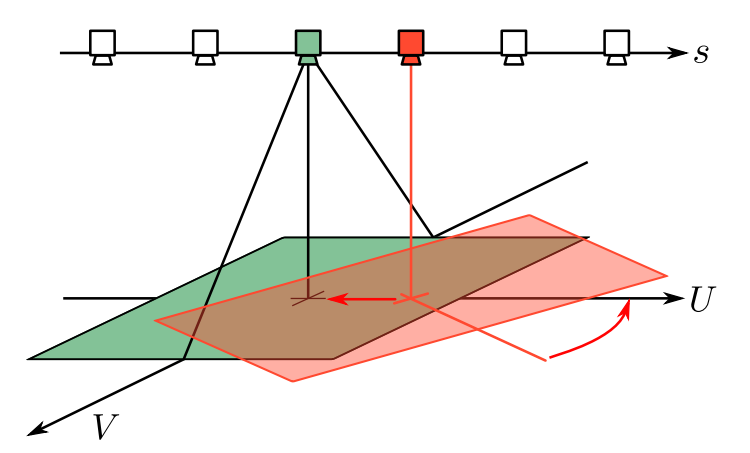
\includegraphics[width=0.8\linewidth]{images/coregistration-principal-rotation}
    \caption{The simplified case of a planar scene and collinear  cameras having only rotations about the principal axes and translations parallel to the scene. Adapted from \protect\bibentry{dansereau2014plenoptic}}
    \label{fig:coregistration-principal-rotation}
\end{figure}

\begin{figure}[H]
    \centering
    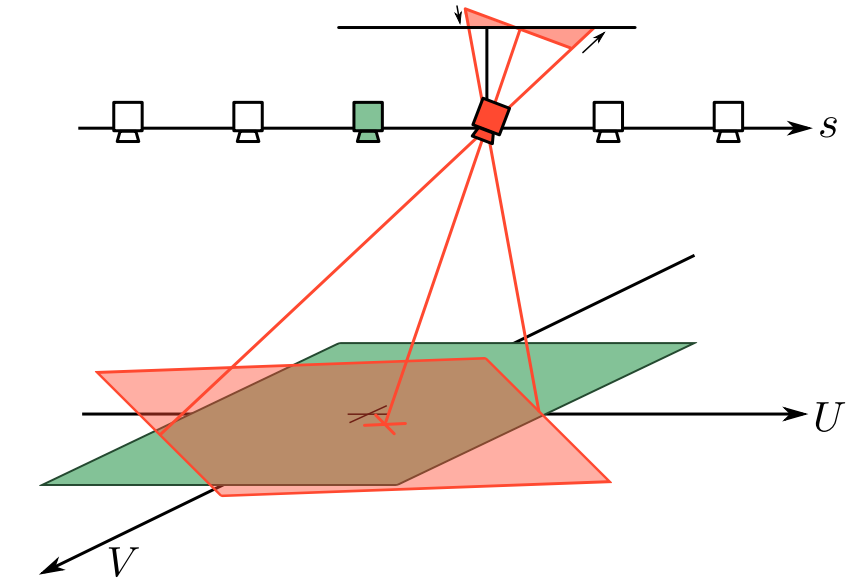
\includegraphics[width=0.8\linewidth]{images/coregistration-arbitrary-rotation}
    \caption{In the case of cameras having arbitrary rotations, images can be reprojected onto a plane parallel with the $U,V$ plane, based on an estimate of the camera's orientation. Adapted from \protect\bibentry{dansereau2014plenoptic}}
    \label{fig:coregistration-arbitrary-rotation}
\end{figure}

\end{document}